% Figure 3: Conformal Selective Triage Decision Flow
% Standalone TikZ -- compiles independently to PDF
\documentclass[tikz,border=10pt]{standalone}
\usepackage{tikz}
\usetikzlibrary{shapes.geometric, arrows.meta, positioning, calc, fit, backgrounds}
\usepackage{amsmath}

% ── Colour palette (consistent across all figures) ──────────────────────────
\definecolor{processblue}{HTML}{4A90D9}
\definecolor{processbluedark}{HTML}{2C6FAC}
\definecolor{alertred}{HTML}{E74C3C}
\definecolor{alertreddark}{HTML}{C0392B}
\definecolor{cleargreen}{HTML}{27AE60}
\definecolor{cleargreendark}{HTML}{1E8449}
\definecolor{deferamber}{HTML}{E67E22}
\definecolor{deferamberdk}{HTML}{CA6F1E}
\definecolor{defergray}{HTML}{7F8C8D}
\definecolor{bglight}{HTML}{F0F4F8}
\definecolor{patientteal}{HTML}{1ABC9C}
\definecolor{patienttealdark}{HTML}{16A085}
\definecolor{textdark}{HTML}{2C3E50}
\definecolor{annocolor}{HTML}{8E44AD}

\begin{document}
\sffamily
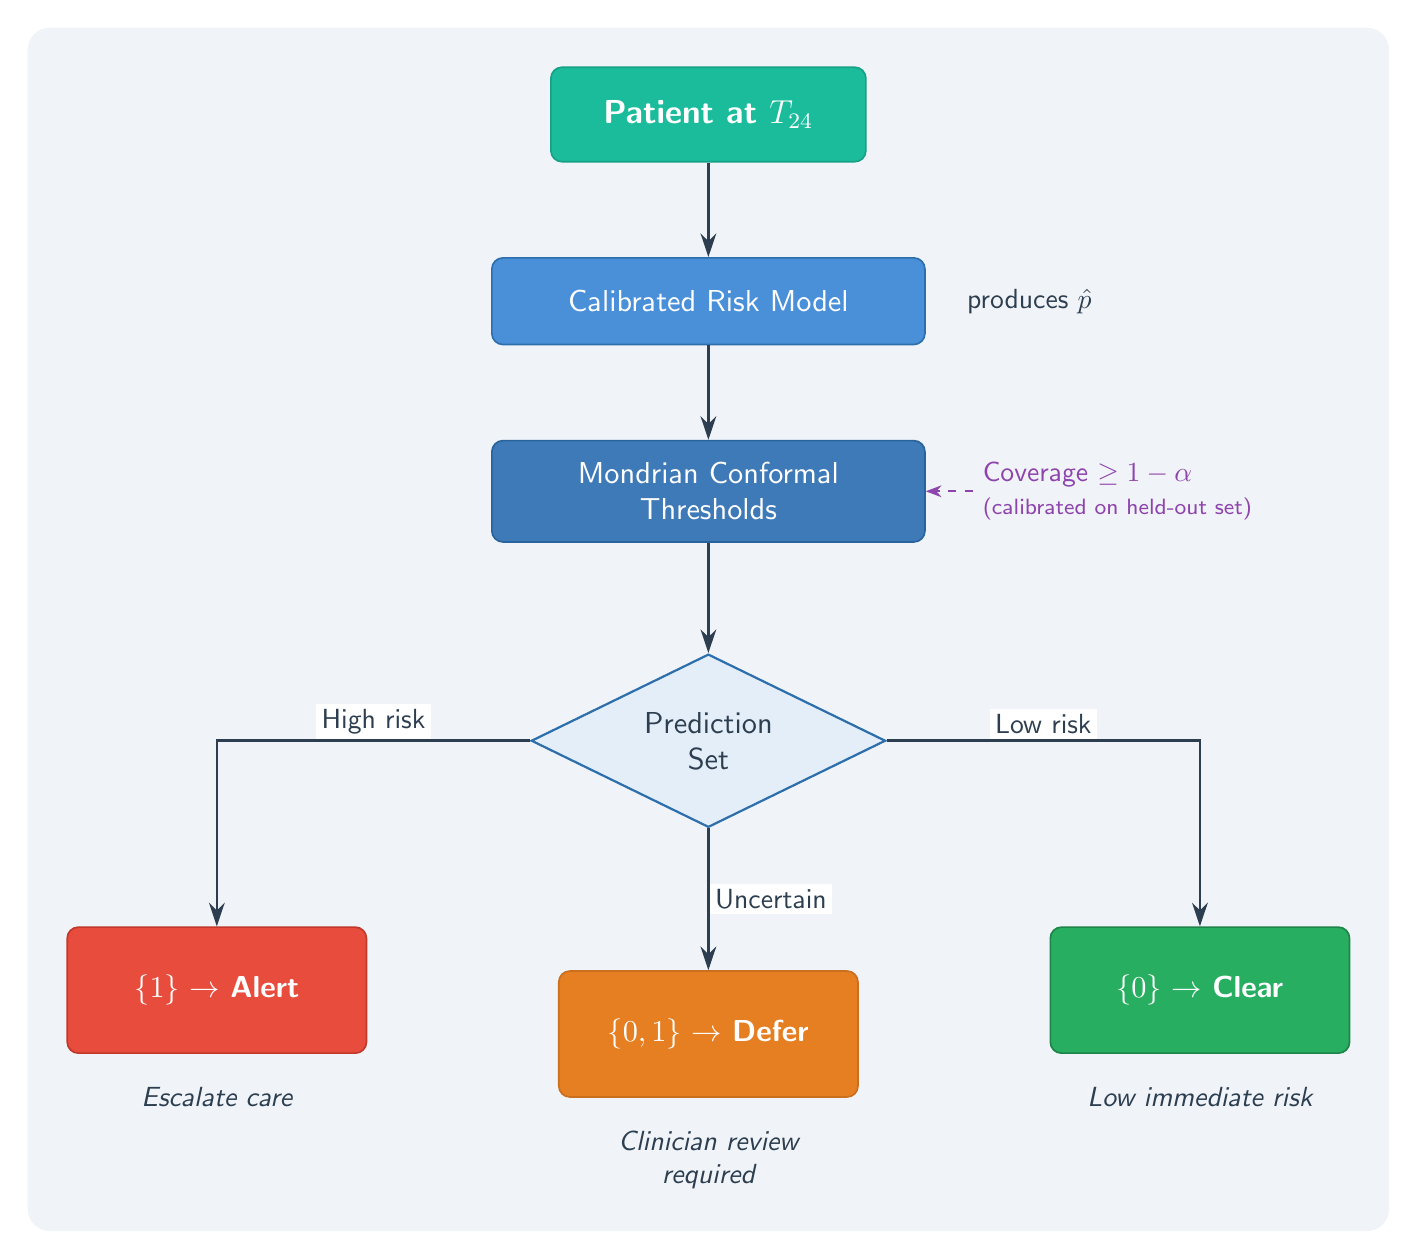
\begin{tikzpicture}[
    % ── Node styles ──────────────────────────────────────────────────────
    base/.style={
        draw, rounded corners=4pt, minimum height=1.1cm,
        font=\fontsize{11}{13}\selectfont\sffamily,
        text=white, align=center, inner sep=8pt,
        line width=0.6pt
    },
    patientnode/.style={
        base, fill=patientteal, draw=patienttealdark,
        minimum width=4cm, minimum height=1.2cm,
        font=\fontsize{12}{14}\selectfont\sffamily\bfseries
    },
    processnode/.style={
        base, fill=processblue, draw=processbluedark,
        minimum width=5.5cm
    },
    threshnode/.style={
        base, fill=processblue!85!black, draw=processbluedark!90!black,
        minimum width=5.5cm
    },
    decision/.style={
        draw, diamond, aspect=2.2, minimum width=4.5cm,
        minimum height=2.2cm, inner sep=4pt,
        fill=processblue!15, draw=processbluedark,
        line width=0.8pt,
        font=\fontsize{11}{13}\selectfont\sffamily,
        text=textdark, align=center
    },
    alertbox/.style={
        base, fill=alertred, draw=alertreddark,
        minimum width=3.8cm, minimum height=1.6cm
    },
    clearbox/.style={
        base, fill=cleargreen, draw=cleargreendark,
        minimum width=3.8cm, minimum height=1.6cm
    },
    deferbox/.style={
        base, fill=deferamber, draw=deferamberdk,
        minimum width=3.8cm, minimum height=1.6cm
    },
    actionlabel/.style={
        font=\fontsize{10}{12}\selectfont\sffamily\itshape,
        text=textdark, align=center
    },
    annotation/.style={
        font=\fontsize{10}{12}\selectfont\sffamily,
        text=annocolor, align=left
    },
    % ── Arrow style ──────────────────────────────────────────────────────
    arr/.style={
        -{Stealth[length=3mm, width=2mm]},
        line width=0.9pt, color=textdark
    },
    arrlabel/.style={
        font=\fontsize{10}{12}\selectfont\sffamily,
        text=textdark, midway, fill=white, inner sep=2pt
    }
]

% ═══════════════════════════════════════════════════════════════════════════
% Vertical flow
% ═══════════════════════════════════════════════════════════════════════════

% 1. Patient
\node[patientnode] (patient) {Patient at $T_{24}$};

% 2. Calibrated risk model
\node[processnode, below=1.2cm of patient] (model)
    {Calibrated Risk Model};

% Probability annotation
\node[right=0.4cm of model, font=\fontsize{10}{12}\selectfont\sffamily,
      text=textdark] (phat) {produces $\hat{p}$};

% 3. Mondrian conformal thresholds
\node[threshnode, below=1.2cm of model] (thresh)
    {Mondrian Conformal\\Thresholds};

% Coverage annotation
\node[annotation, right=0.6cm of thresh] (coverage)
    {Coverage $\geq 1 - \alpha$\\{\footnotesize (calibrated on held-out set)}};
\draw[annocolor, dashed, line width=0.6pt, -{Stealth[length=2mm]}]
    (coverage.west) -- (thresh.east);

% 4. Decision diamond
\node[decision, below=1.4cm of thresh] (decide)
    {Prediction\\Set};

% ═══════════════════════════════════════════════════════════════════════════
% Three outcome branches
% ═══════════════════════════════════════════════════════════════════════════

% Left — Alert
\node[alertbox, below left=1.8cm and 3.2cm of decide] (alert)
    {$\{1\}$ $\rightarrow$ \textbf{Alert}};
\node[actionlabel, below=0.3cm of alert] {Escalate care};

% Centre — Defer
\node[deferbox, below=1.8cm of decide] (defer)
    {$\{0,1\}$ $\rightarrow$ \textbf{Defer}};
\node[actionlabel, below=0.3cm of defer] {Clinician review\\required};

% Right — Clear
\node[clearbox, below right=1.8cm and 3.2cm of decide] (clear)
    {$\{0\}$ $\rightarrow$ \textbf{Clear}};
\node[actionlabel, below=0.3cm of clear] {Low immediate risk};

% ═══════════════════════════════════════════════════════════════════════════
% Arrows
% ═══════════════════════════════════════════════════════════════════════════
\draw[arr] (patient) -- (model);
\draw[arr] (model)   -- (thresh);
\draw[arr] (thresh)  -- (decide);

% Diamond to outcomes
\draw[arr] (decide.west)  -| (alert.north)
    node[arrlabel, pos=0.25, above] {High risk};
\draw[arr] (decide.south) -- (defer.north)
    node[arrlabel, right] {Uncertain};
\draw[arr] (decide.east)  -| (clear.north)
    node[arrlabel, pos=0.25, above] {Low risk};

% ═══════════════════════════════════════════════════════════════════════════
% Background
% ═══════════════════════════════════════════════════════════════════════════
\coordinate (bottompad) at ([yshift=-1.2cm]defer.south);
\begin{scope}[on background layer]
    \node[fill=bglight, rounded corners=8pt, inner sep=14pt,
          fit=(patient)(alert)(clear)(defer)(coverage)(bottompad)] {};
\end{scope}

\end{tikzpicture}
\end{document}
